\section*{ÔN TẬP KIỂM TRA GIỮA KÌ 1 - ĐỀ 02}
\setcounter{ex}{0}\setcounter{bt}{0}
\noindent{\bf\fontfamily{qag}\selectfont\color{violet}A. PHẦN TRẮC NGHIỆM}
\Opensolutionfile{ans}[ans/ans-0-GK1-CanhDieu-De2-NH23-24]
\begin{ex}%[Dự Án 6 -Đề GHK1 - Khối 10]%[Dương Văn Đức]%[0C1Y1-1]
Phát biểu nào sau đây là một mệnh đề toán học?
\choice
{Trận đấu bóng rổ này hay quá!}
{An Giang là tỉnh thuộc miền Tây Nam Bộ}
{\True $5$ là một số nguyên}
{Hôm nay bạn có học môn Anh không?}
\loigiai{
$5$ là một số nguyên là một mệnh đề toán học.
}
\end{ex}
\begin{ex}%[Dự Án 6 -Đề GHK1 - Khối 10]%[Dương Văn Đức]%[0C1Y1-3]
Phủ định của mệnh đề \lq\lq$\sqrt{5}>3$\rq\rq\, là
\choice
{$\sqrt{5}=3$}
{$\sqrt{5} \geq 3$}
{$\sqrt{5}<3$}
{\True $\sqrt{5} \leq 3$}
\loigiai{
Phủ định của mệnh đề \lq\lq $\sqrt{5}>3$\rq\rq\, là \lq\lq $\sqrt{5} \leq 3$\rq\rq.
}
\end{ex}
\begin{ex}%[Dự Án 6 -Đề GHK1 - Khối 10]%[Dương Văn Đức]%[0C1Y2-1]
Hãy liệt kê các phần tử của tập hợp $A=\{x \in \mathbb{N} \mid x<\sqrt{7}\}$.
\choice
{$A=\{0 ; 1 ; 2 ; 3\}$}
{\True $A=\{0 ; 1 ; 2\}$}
{$A=\{0 ; 1 ; 2 ; 3 ; 4 ; 5 ; 6\}$}
{$A=\{1 ; 2\}$}
\loigiai{
Ta có $\sqrt{7}\approx 2,64$ nên  $A=\{x \in \mathbb{N} \mid x<\sqrt{7}\}=\{0;1;2\}$.
}
\end{ex}
\begin{ex}%[Dự Án 6 -Đề GHK1 - Khối 10]%[Dương Văn Đức]%[0C1Y2-2]
Tập hợp nào sau đây là tập con của tập hợp $A=\{0; 1; 2; 3\}$?
\choice
{$\{0; 1; 2; 4\}$}
{\True $\{0; 1\}$}
{$\{0; 1;-1\}$}
{$\{0; 1; 2; 3;-1\}$}
\loigiai{
Ta thấy $0 \in A$; $1 \in A \Rightarrow\{0; 1\} \subset A$.
}
\end{ex}
\begin{ex}%[Dự Án 6 -Đề GHK1 - Khối 10]%[Dương Văn Đức]%[0C1Y2-6] 
Sử dụng các kí hiệu khoảng, đoạn để viết tập hợp $A=\{x \in \mathbb{R} \mid 4 \leq x \leq 9\}$.
\choice
{\True $A=[4; 9]$}
{$A=(4; 9]$}
{$A=[4; 9)$}
{$A=(4; 9)$}
\loigiai{
Ta có $A=\{x \in \mathbb{R} \mid 4 \leq x \leq 9\}\Leftrightarrow A=[4; 9]$.
}
\end{ex}
\begin{ex}%[Dự Án 6 -Đề GHK1 - Khối 10]%[Dương Văn Đức]%[0C1Y2-6]
Cho $X=\{7; 2; 8; 4; 9; 12\}$; $Y=\{1; 3; 7; 4\}$. Tập nào sau đây bằng tập $X\cap Y$?
\choice
{$\{1; 2; 3; 4; 8; 9; 7; 12\}$}
{$\{2; 8; 9; 12\}$}
{\True $\{4; 7\}$}
{$\{1; 3\}$}
\loigiai{
Ta có
$X=\{7; 2; 8; 4; 9; 12\}$, $Y=\{1; 3; 7; 4\} \Rightarrow X \cap Y=\{7; 4\}$.
}
\end{ex}
\begin{ex}%[Dự Án 6 -Đề GHK1 - Khối 10]%[Dương Văn Đức]%[0C1Y1-2]
Trong các mệnh đề sau, tìm mệnh đề sai?
\choice
{\True $A \in A$}
{$\varnothing \subset A$}
{$A \subset A$}
{$A \neq\{A\}$}
\loigiai{
\begin{itemize}
\item $A \in A$ sai do tập $A$ thì không thể là phần tử của tập $A$ (sai ký hiệu).
\item $\varnothing \subset A$ đúng do tập $\varnothing$ là tập con của mọi tập hợp.
\item $A \subset A$ đúng do tập $A$ là tập con của chính nó.
\item $A \neq\{A\}$ đúng do tập hợp có chứa một phần tử $\{A\}$ thì không thể bằng tập $A$.
\end{itemize}
}
\end{ex}
\begin{ex}%[Dự Án 6 -Đề GHK1 - Khối 10]%[Dương Văn Đức]%[0C2Y1-2]
Câu nào sau đây đúng?\\
Miền nghiệm của bất phương trình $3(x-1)+4(y-2)<5 x-3$ là nửa mặt phẳng chứa điểm
\choice
{\True $(0 ; 0)$}
{$(-4 ; 2)$}
{$(-2 ; 2)$}
{$(-5 ; 3)$}
\loigiai{
Ta có \allowdisplaybreaks
\begin{eqnarray*}
3(x-1)+4(y-2)<5 x-3 &\Leftrightarrow& 3x-3+4 y-8<5 x-3\\ &\Leftrightarrow& 2 x-4 y+8>0\\
&\Leftrightarrow& x-2 y+4>0.
\end{eqnarray*}
Dễ thấy tại điểm $(0 ; 0)$ ta có $0-2\cdot0+4=4>0$.
}
\end{ex}
\begin{ex}%[Dự Án 6 -Đề GHK1 - Khối 10]%[Dương Văn Đức]%[0C2Y1-2]
Cặp số nào sau đây là nghiệm của hệ bất phương trình $\heva{&x+y>-3 \\& -x+2 y<3}$?
\choice
{\True $(1 ; 0)$}
{$(-5 ; 0)$}
{$(-2 ;-3)$}
{$(0 ;-5)$}
\loigiai{
Thay $x=1$; $y=0$ vào hai bất phương trình của hệ ta có
$\heva{&1+0>-3\\&-1+2\cdot 0<3}$ là mệnh đề đúng.\\
Vậy $(1 ; 0)$ là nghiệm của hệ bất phương trình.
}
\end{ex}
\begin{ex}%[Dự Án 6 -Đề GHK1 - Khối 10]%[Dương Văn Đức]%[0C2Y1-2]
Cặp số nào sau đây không là nghiệm của hệ bất phương trình $\heva{&x+y\leq 3\\&x-2y>-2}$?
\choice
{$(0;0)$}
{$(1;1)$}
{\True $(-1;1)$}
{$(-1;0)$}
\loigiai{
Thay $x=-1$; $y=1$ vào hai bất phương trình của hệ ta có $\heva{&-1+1\le 3\\& -1-2\cdot 1>-2}$ là mệnh đề sai.\\
Vậy $(-1;1)$  không là nghiệm của hệ bất phương trình.
}
\end{ex}
\begin{ex}%[Dự Án 6 -Đề GHK1 - Khối 10]%[Dương Văn Đức]%[0C2Y2-3]
Miền nghiệm của hệ bất phương trình $\heva{&2 x-5y>1 \\& x+y>-5 \\& x-2y \geq-3}$ là phần mặt phẳng chứa điểm có tọa độ là
\choice
{$(0; 0)$}
{\True $(1; 0)$}
{$(0; 2)$}
{$(0; 3)$}
\loigiai{
Thay $x=1$; $y=0$ vào ba bất phương trình của hệ ta có
$\heva{&2\cdot1-5\cdot0>1\\&1+0>-5\\&1-2\cdot0 \geq-3}$
là mệnh đề đúng.\\
Vậy miền nghiệm của hệ bất phương trình là phần mặt phẳng chứa điểm có toạ độ $(1; 0)$.
}
\end{ex}
\begin{ex}%[Dự Án 6 -Đề GHK1 - Khối 10]%[Dương Văn Đức]%[0C4Y1-2]
Tính $\sin 30^{\circ}$.
\choice
{\True $\dfrac{1}{2}$}
{$\dfrac{2}{3}$}
{$0$}
{$-0{,}988$}
\loigiai{Ta có $\sin 30^{\circ}=\dfrac{1}{2}$.}
\end{ex}
\begin{ex}%[Dự Án 6 -Đề GHK1 - Khối 10]%[Dương Văn Đức]%[0C4Y2-1]
Cho tam giác $ABC$ có $a=8$, $b=10$, góc $C$ bằng $60^{\circ}$. Độ dài cạnh $c$ là?
\choice
{$c=3\sqrt{21}$}
{$c=7\sqrt{2}$}
{$c=2\sqrt{11}$}
{\True $c=2\sqrt{21}$}
\loigiai{
Ta có $c^2=a^2+b^2-2 ab\cos C=8^2+10^2-2 \cdot 8 \cdot 10 \cdot \cos 60^{\circ}=84 \Rightarrow c=2 \sqrt{21}$.
}
\end{ex}
\begin{ex}%[Dự Án 6 -Đề GHK1 - Khối 10]%[Dương Văn Đức]%[0C4Y2-1]
Trong mặt phẳng, cho tam giác $ABC$ có $AC=4$ cm, góc $A=60^{\circ}$, $B=45^{\circ}$. Độ dài cạnh $BC$ là
\choice
{\True $2\sqrt{6}$}
{$2+2\sqrt{3}$}
{$2\sqrt{3}-2$}
{$\sqrt{6}$}
\loigiai{
Ta có $\dfrac{BC}{\sin A}=\dfrac{AC}{\sin B} \Leftrightarrow BC=\dfrac{AC\cdot\sin A}{\sin B}=\dfrac{4 \cdot \dfrac{\sqrt{3}}{2}}{\dfrac{\sqrt{2}}{2}}=2 \sqrt{6}$.
}
\end{ex}
\begin{ex}%[Dự Án 6 -Đề GHK1 - Khối 10]%[Dương Văn Đức]%[0C4Y2-1]
Cho tam giác $ABC$ thoả mãn hệ thức $b+c=2a$. Trong các mệnh đề sau, mệnh đề nào đúng?
\choice
{$\cos B+\cos C=2\cos A$}
{\True $\sin B+\sin C=2\sin A$}
{$\sin B+\sin C=\dfrac{1}{2}\sin A$}
{$\sin B+\cos C=2 \sin A$}
\loigiai{
Theo định lý sin ta có $a=2R\sin A$; $b=2R\sin B$; $c=2R\sin C$.\\
Theo bài ra ta có 
\allowdisplaybreaks
\begin{eqnarray*}
b+c=2a&\Leftrightarrow& 2R\sin A+2R\sin B=2\cdot 2R\sin A\\
&\Leftrightarrow& 2R\left( \sin B+\sin C\right)=4R\sin A\\
&\Leftrightarrow&\sin B+\sin C=2\sin A.
\end{eqnarray*}
}
\end{ex}
\begin{ex}%[Dự Án 6 -Đề GHK1 - Khối 10]%[Dương Văn Đức]%[0C4B2-1]
Gọi $S=m_a^2+m_b^2+m_c^2$ là tổng bình phương độ dài ba trung tuyến của tam giác $ABC$. Trong các mệnh đề sau mệnh đề nào đúng?
\choice
{\True $S=\dfrac{3}{4}\left(a^2+b^2+c^2\right)$}
{$S=a^2+b^2+c^2$}
{$S=\dfrac{3}{2}\left(a^2+b^2+c^2\right)$}
{$S=3\left(a^2+b^2+c^2\right)$}
\loigiai{
Ta có $S=m_a^2+m_b^2+m_c^2=\dfrac{b^2+c^2}{2}-\dfrac{a^2}{4}+\dfrac{a^2+c^2}{2}-\dfrac{b^2}{4}+\dfrac{a^2+b^2}{2}-\dfrac{c^2}{4}=\dfrac{3}{4}\left(a^2+b^2+c^2\right)$.
}
\end{ex}
\begin{ex}%[Dự Án 6 -Đề GHK1 - Khối 10]%[Dương Văn Đức]%[0C4B3-1]
Cho lục giác đều $ABCDEF$ tâm $O$. Số các vectơ khác vectơ-không, có điểm đầu điểm cuối lấy từ $7$ điểm $A$, $B$, $C$, $D$, $E$, $F$, $O$ là
\choice
{$21$}
{\True $42$}
{$7$}
{$9$}
\loigiai{
\begin{itemize}
\item Các vectơ có điểm đầu là $A$ gồm $\overrightarrow{AB}$, $\overrightarrow{AC}$, $ \overrightarrow{AD}$, $\overrightarrow{AE}$, $\overrightarrow{AF}$, $\overrightarrow{AO}$ (Có 6 vectơ).
\item Tương tự số vectơ có điểm đầu là $B$, $C$, $D$, $E$, $F$, $O$ cũng là $6$ vectơ.
\item Vậy từ $7$ điểm $A$, $B$, $C$, $D$, $E$, $F$, $O$ có thể tạo được $7\cdot6=42$ vectơ thỏa mãn yêu cầu.
\end{itemize}
}
\end{ex}
\begin{ex}%[Dự Án 6 -Đề GHK1 - Khối 10]%[Dương Văn Đức]%[0C4B3-3]
Cho tam giác $ABC$ có $M$, $N$, $P$ lần lượt là trung điểm của $AB$, $BC$, $CA$. Khẳng định nào sau đây là đúng?
\choice
{$\overrightarrow{MN}=\overrightarrow{CP}$ và $\overrightarrow{MP}=\overrightarrow{NC}$}
{\True $\overrightarrow{MN}=\overrightarrow{PC}$ và $\overrightarrow{MP}=\overrightarrow{NC}$}
{$\overrightarrow{MN}=\overrightarrow{CP}$ và $\overrightarrow{MP}=\overrightarrow{CN}$}
{$\overrightarrow{MN}=\overrightarrow{CP}$ và $\overrightarrow{MP}=\overrightarrow{NC}$}
\loigiai{
\begin{center}
\begin{tikzpicture}[>=stealth,line join=round,line cap=round,font=\footnotesize,scale=1,declare function={a=3;b=4;g=60;}]
\path (0,0)coordinate(B)
(60:a)coordinate(A)
(b,0)coordinate(C)
($(A)!1/2!(B)$)coordinate (M)
($(C)!1/2!(B)$)coordinate (N)
($(A)!1/2!(C)$)coordinate (P)
;
\draw (A)--(B)--(C)--cycle;
\draw (M)--(N)--(P)--cycle;
\foreach \i \g in {A/90,B/-90,C/-90,M/130,N/-90,P/60}\fill(\i)circle(1pt)+(\g:.25)node{$\i$};
\end{tikzpicture}
\end{center}
Theo hình vẽ ta có $MNCP$ là hình bình hành suy ra $\overrightarrow{MN}=\overrightarrow{PC}$ và $\overrightarrow{MP}=\overrightarrow{NC}$.
}
\end{ex}
\begin{ex}%[Dự Án 6 -Đề GHK1 - Khối 10]%[Dương Văn Đức]%[0C4Y4-1]
Cho hai tam giác $BCD$ và $B'C'D'$ có chung trọng tâm $G$. Tổng $\overrightarrow{B'B}+\overrightarrow{C'C}+\overrightarrow{D'D}$ bằng
\choice
{$\overrightarrow{BB'}$}
{\True $\overrightarrow{0}$}
{$\overrightarrow{B'B}$}
{$\overrightarrow{BC'}$}
\loigiai{
Ta có 
\allowdisplaybreaks
\begin{eqnarray*}
\overrightarrow{B'B}+\overrightarrow{C'C}+\overrightarrow{D'D}&=&\overrightarrow{B'G}+\overrightarrow{GB}+\overrightarrow{C'G}+\overrightarrow{GC}+\overrightarrow{D'G}+\overrightarrow{GD}\\
&=&-\left(\overrightarrow{G B'}+\overrightarrow{G C'}+\overrightarrow{G D'}\right)+(\overrightarrow{GB}+\overrightarrow{GC}+\overrightarrow{GD})\\
&=&\overrightarrow{0}+\overrightarrow{0}\\
&=&\overrightarrow{0}.
\end{eqnarray*}
}
\end{ex}
\begin{ex}%[Dự Án 6 -Đề GHK1 - Khối 10]%[Dương Văn Đức]%[0C4B4-5]
Cho tam giác $ABC$ đều cạnh $a$, $H$ là trung điểm cạnh $BC$. Tính $\left|\overrightarrow{CH}+\overrightarrow{HA}\right|$.
\choice
{$\left|\overrightarrow{CH}+\overrightarrow{HA}\right|=\dfrac{a}{2}$}
{$\left|\overrightarrow{CH}+\overrightarrow{HA}\right|=\dfrac{3 a}{2}$}
{$\left|\overrightarrow{CH}+\overrightarrow{HA}\right|=\dfrac{\sqrt{3}a}{2}$}
{\True $\left|\overrightarrow{CH}+\overrightarrow{HA}\right|=a$}
\loigiai{
Ta có $\left|\overrightarrow{CH}+\overrightarrow{HA}\right|=\left|\overrightarrow{CA}\right|=AC=a$.
}
\end{ex}
\begin{ex}%[Dự Án 6 -Đề GHK1 - Khối 10]%[Dương Văn Đức]%[0C1B1-2]
Trong các mệnh đề sau, mệnh đề nào đúng?
\choice
{\True $\exists x \in \mathbb{Q}\colon 9x^2-1=0$}
{$\forall x \in \mathbb{R}\colon x^2+2x+1>0$}
{$\forall n \in \mathbb{N}\colon n^2>n$}
{$\exists n \in \mathbb{Z}\colon n^2-3n-5=0$}
\loigiai{
\begin{itemize}
\item $9x^2-1=0\Leftrightarrow x=\pm \dfrac{1}{3}\in \mathbb{Q}$ suy ra mệnh đề \lq\lq$\exists x \in \mathbb{Q}\colon 9x^2-1=0$\rq\rq\, đúng.
\item $\forall x \in \mathbb{R}\colon x^2+2x+1>0$ sai vì  tồn tại $x=-1$ nhưng $x^2+2x+1=0$.
\item $\forall n \in \mathbb{N}\colon n^2>n$ sai vì tồn tại $n=1$ nhưng $1^2=1$.
\item $\exists n \in \mathbb{Z}\colon n^2-3n-5=0$ sai vì $n^2-3 n-5=0 \Leftrightarrow n=\dfrac{3 \pm \sqrt{29}}{2} \notin \mathbb{Z}$.
\end{itemize}
}
\end{ex}
\begin{ex}%[Dự Án 6 -Đề GHK1 - Khối 10]%[Dương Văn Đức]%[0C1Y2-6]
Cho tập hợp $A=(0; 6]$ và $B=(-3; 5)$. Khi đó $A \cup B$ bằng
\choice
{$(0; 5)$}
{\True $(-3; 6]$}
{$(-3; 0)$}
{$(5; 6]$}
\loigiai{
Ta có $A=(0; 6]$ và $B=(-3; 5)$ nên $A \cup B=(-3; 6]$.
}
\end{ex}
\begin{ex}%[Dự Án 6 -Đề GHK1 - Khối 10]%[Dương Văn Đức]%[0C1B2-5]
Một lớp có $25$ học sinh giỏi môn Toán, $23$ học sinh giỏi môn Văn, $14$ học sinh giỏi cả môn Toán và Văn, có $6$ học sinh không học giỏi môn nào cả. Hỏi lớp đó có bao nhiêu học sinh?
\choice
{$54$}
{\True $40$}
{$26$}
{$68$}
\loigiai{
Gọi $T$ là tập hợp các học sinh giỏi môn Toán và $V$ là tập hợp các học sinh giỏi môn Văn.\\
Gọi $n(T)$ là số học sinh giỏi môn Toán, $n(V)$ là số học sinh giỏi môn Toán, $n(T \cap V)$ là số học sinh giỏi cả Toán và Văn, $n(T \cup V)$ là số học sinh giỏi Toán hoặc Văn.\\
Ta có số học sinh của lớp là $n(T \cup V)+6$.\\
Mà $n(T \cup V)=n(T)+n(V)-n(T \cap V)=25+23-14=34$.\\
Vậy số học sinh của lớp là $34+6=40$.
}
\end{ex}
\begin{ex}%[Dự Án 6 -Đề GHK1 - Khối 10]%[Dương Văn Đức]%[0C2B1-2]
Tìm giá trị của tham số $m$ sao cho $\heva{&x=1 \\& y=2}$ là nghiệm của bất phương trình $mx+(m+1)y>5$.
\choice
{$m=1$}
{\True $m>1$}
{$m<1$}
{$m \neq 1$}
\loigiai{
Ta có $\heva{&x=1 \\& y=2}$ là nghiệm của bất phương trình $m x+(m+1) y>5$ khi và chỉ khi:
\[
m\cdot1+(m+1)\cdot2>5 \Leftrightarrow 3m>3 \Leftrightarrow m>1.
\]
}
\end{ex}
\begin{ex}%[Dự Án 6 -Đề GHK1 - Khối 10]%[Dương Văn Đức]%[0C2K1-2]
Miền nghiệm (phần không bị gạch chéo) của bất phương trình $3 x+2y>6$ là
\choice
{\True \begin{tikzpicture}[>=stealth,line join=round,line cap=round,font=\footnotesize,scale=.8,every node/.style={scale=0.9},declare function={
a=3;b=2;c=-6;
f(\x)=-c/b-a/b*(\x);}]
\begin{scope}
\clip (-3,-2) rectangle (4,4.5);
\draw[dotted] (-3,-2) rectangle (4,4.5);
\fill[pattern=north west lines,] plot[domain=-3:4.5] (\x,{f(\x)})--(-3,-4.5)--cycle; 
\draw[thick,samples=150,smooth,domain=-7:7] plot(\x,{f(\x)});
\end{scope}
\draw[->] (-3,0)--(4,0)node[above]{$x$};
\draw[->] (0,-2)--(0,4.5)node[left]{$y$};
\fill (0,0)circle(1.5pt)node[above right]{$O$}
(2,0)circle(1.5pt) (2.1,0)node[above]{$2$}
(0,3)circle(1.5pt)node[right]{$3$}
;
\end{tikzpicture}}
{\begin{tikzpicture}[>=stealth,line join=round,line cap=round,font=\footnotesize,scale=.8,every node/.style={scale=0.9},declare function={
a=3;b=-2;c=6;
f(\x)=-c/b-a/b*(\x);}]
\begin{scope}
\clip (-3,-2) rectangle (4,4.5);
\draw[dotted] (-3,-2) rectangle (4,4.5);
\fill[pattern=north west lines,] plot[domain=-3:4.5] (\x,{f(\x)})--(4,4.5)--(4,-2)-|cycle; 
\draw[thick,samples=150,smooth,domain=-7:7] plot(\x,{f(\x)});
\end{scope}
\draw[->] (-3,0)--(4,0)node[above]{$x$};
\draw[->] (0,-2)--(0,4.5)node[left]{$y$};
\fill (0,0)circle(1.5pt)node[above right]{$O$}
(-2,0)circle(1.5pt) (-2.1,0)node[above]{$-2$}
(0,3)circle(1.5pt)node[left]{$3$}
;
\end{tikzpicture}}
{\begin{tikzpicture}[>=stealth,line join=round,line cap=round,font=\footnotesize,scale=.8,every node/.style={scale=0.9},declare function={f(\x)=3/2*(\x)+3;}]
\begin{scope}
\clip (-3,-2) rectangle (4,4.5);
\draw[dotted] (-3,-2) rectangle (4,4.5);
\fill[pattern=north west lines] plot[domain=-3:4.5] (\x,{f(\x)})--(-3,4.5)--cycle; 
\draw[thick,samples=150,smooth,domain=-7:7] plot(\x,{f(\x)});
\end{scope}
\draw[->] (-3,0)--(4,0)node[above]{$x$};
\draw[->] (0,-2)--(0,4.5)node[left]{$y$};
\fill (0,0)circle(1.5pt)node[above right]{$O$}
(-2,0)circle(1.5pt) (-1.9,0)node[below]{$-2$}
(0,3)circle(1.5pt) (0,2.9)node[right]{$3$}
;
\end{tikzpicture}}
{\begin{tikzpicture}[>=stealth,line join=round,line cap=round,font=\footnotesize,scale=.8,every node/.style={scale=0.9},declare function={
a=3;b=2;c=6;
f(\x)=-c/b-a/b*(\x);}]
\begin{scope}
\clip (-4,-4) rectangle (2,2);
\draw[dotted] (-4,-4) rectangle (2,2);
\fill[pattern=north west lines] plot[domain=-4:4.5] (\x,{f(\x)})--(4,-4)-|(-4,2)--cycle; 
\draw[thick,samples=150,smooth,domain=-5:5] plot(\x,{f(\x)});
\end{scope}
\draw[->] (-4,0)--(2,0)node[above]{$x$};
\draw[->] (0,-4)--(0,2)node[left]{$y$};
\fill (0,0)circle(1.5pt)node[above right]{$O$}
(-2,0)circle(1.5pt) (-1.9,0)node[above]{$-2$}
(0,-3)circle(1.5pt)node[right]{$-3$}
;
\end{tikzpicture}}
\loigiai{
Ta có đường thẳng $d\colon 3x+2y=6$ đi qua điểm $(2;0)$, $(3;0)$.
}
\end{ex}
\begin{ex}%[Dự Án 6 -Đề GHK1 - Khối 10]%[Dương Văn Đức]%[0C2K2-3]
Miền nghiệm của hệ bất phương trình $\heva{&-x+4 y>0 \\& -2 x+y<0 \\& x+3 y<7 \\& x<3}$ là
\choice
{Một nửa mặt phẳng}
{Miền tam giác}
{\True Miền tứ giác}
{Miền ngũ giác}
\loigiai{
\begin{center}
\begin{tikzpicture}[>=stealth,line join=round,line cap=round,font=\footnotesize,scale=.8,every node/.style={scale=0.9},declare function={
f(\x)=(\x)/4;
g(\x)=2*(\x);
h(\x)=7/3-1/3*(\x);
}]
\begin{scope}
\clip (-1,-1) rectangle (5,4);
\fill[pattern=north west lines,] (0,0)--(3,{f(3)})--(3,{h(3)})--(1,2)--cycle;
\draw[thick,samples=150,smooth,domain=-7:7] plot(\x,{f(\x)});
\draw[thick,samples=150,smooth,domain=-7:7,red] plot(\x,{g(\x)});
\draw[thick,samples=150,smooth,domain=-7:7,blue] plot(\x,{h(\x)});
\draw[thick] (3,-2)--(3,5)node[right,pos=.8]{$d_4$};
\end{scope}
\draw[->] (-1,0)--(5,0)node[below]{$x$};
\draw[->] (0,-1)--(0,4)node[left]{$y$};
\fill (0,0)circle(1.5pt)node[below right]{$O$}
(3,{h(3)})circle(1.5pt) node[xshift=1ex,yshift=1ex]{$B$}
(3,{f(3)})circle(1.5pt)node[right,yshift=-1ex]{$A$}
(1,2)circle(1.5pt)node[xshift=-.5ex,yshift=1.2ex]{$C$}
;
\draw[dashed]
(0,2)node[left]{$2$}-|(1,0)node[below]{$1$}
(0,1)node[left]{$1$}-|(4,0)node[below]{$4$}
;
\path (-.5,{h(-1.5)})node{$d_3$}
(1.7,{g(2)})node{$d_2$}
(4.5,{f(5.3)})node{$d_1$}
;
\end{tikzpicture}
\end{center}
Miền nghiệm của hệ bất phương trình đã cho là miền tứ giác $OABC$.
}
\end{ex}
\begin{ex}%[Dự Án 6 -Đề GHK1 - Khối 10]%[Dương Văn Đức]%[0C2K2-3]
Phần không gạch chéo ở hình sau đây là biểu diễn miền nghiệm của hệ bất phương trình nào trong bốn hệ bất phương trình dưới đây?
\begin{center}
\begin{tikzpicture}[>=stealth,line join=round,line cap=round,font=\footnotesize,scale=.8,every node/.style={scale=0.9},declare function={
a=3;b=2;c=-6;
f(\x)=-c/b-a/b*(\x);}]
\begin{scope}
\clip (-3,-2) rectangle (4,4.5);
\fill[pattern=north west lines,] (-3,-2) rectangle (4,4.5);
\fill[white] (-3,0)--(2,0)--(-1,4.5)-|cycle;
\draw[thick,samples=150,smooth,domain=-7:7] plot(\x,{f(\x)});
\end{scope}
\draw[->] (-3,0)--(4,0)node[above]{$x$};
\draw[->] (0,-2)--(0,4.5)node[left]{$y$};
\fill (0,0)circle(1.5pt)node[above right]{$O$}
(2,0)circle(1.5pt) (2.1,0)node[above]{$2$}
(0,3)circle(1.5pt)node[left]{$3$};
\end{tikzpicture}
\end{center}
\choice
{\True $\heva{&y>0 \\& 3x+2y<6}$}
{$\heva{&y>0 \\& 3x+2y<-6}$}
{$\heva{&x>0 \\& 3x+2y<6}$}
{$\heva{&x>0 \\& 3x+2y>-6}$}
\loigiai{
Dựa vào hình vẽ ta thấy đồ thị gồm hai đường thẳng $\left(d_1\right)\colon y=0$ và đường thẳng $\left(d_2\right)\colon 3 x+2y=6$.\\
Miền nghiệm gồm phần $y$ nhận giá trị dương.\\
Lại có $(0;0)$ thỏa mãn bất phương trình $3x+2y<6$ nên hệ bất phương trình là $\heva{&y>0 \\& 3x+2y<6.}$
}
\end{ex}
\begin{ex}%[Dự Án 6 -Đề GHK1 - Khối 10]%[Dương Văn Đức]%[0C2B2-3]
Miền nghiệm của hệ bất phương trình $\heva{&2x+3y-6<0 \\& x \geq 0 \\& 2x-3y-1 \leq 0}$ chứa điểm nào sau đây?
\choice
{$A(1;2)$}
{$B(0;2)$}
{$C(-1;3)$}
{\True $D\left(0;-\dfrac{1}{3}\right)$}
\loigiai{
Trước hết, ta vẽ ba đường thẳng: $\left(d_1\right)\colon 2x+3 y-6=0$; $\left(d_2\right)\colon x=0$; $\left( d_3\right)\colon 2x-3y-1=0$.
\begin{center}
\begin{tikzpicture}[>=stealth,line join=round,line cap=round,font=\footnotesize,scale=.8,every node/.style={scale=0.9},declare function={
a=2;b=3;c=-6;
f(\x)=-c/b-a/b*(\x);g(\x)=2/3*(\x)-1/3;
}]
\begin{scope}
\clip (-3,-2) rectangle (4,4.5);
\draw[dotted] (-3,-2) rectangle (4,4.5);
\fill[pattern=north west lines,] plot[domain=-7:7] (\x,{f(\x)})--(7,7)--cycle; 
\fill[pattern=vertical lines,] plot[domain=-7:7] (\x,{g(\x)})--(7,-7)--cycle; 
\fill[pattern=north east lines,pattern color=blue] (-3,-2) rectangle (0,4.5);
\draw[thick,samples=150,smooth,domain=-7:7] plot(\x,{f(\x)});
\draw[thick,samples=150,smooth,domain=-7:7,blue] plot(\x,{g(\x)});
\end{scope}
\draw[->] (-3,0)--(4,0)node[above]{$x$};
\draw[->] (0,-2)--(0,4.5)node[left]{$y$};
\fill (0,0)circle(1.5pt)node[above right]{$O$}
(3,0)circle(1.5pt) (3.1,0)node[above]{$3$}
(0,2)circle(1.5pt)node[right]{$2$}
(0,-1/3)circle(1.5pt)node[right]{$-\tfrac{1}{3}$};
;
\end{tikzpicture}
\end{center}
Ta thấy $(1;1)$ là nghiệm của cả ba bất phương trình. Điều này có nghĩa là điểm $(1;1)$ thuộc
cả ba miền nghiệm của ba bất phương trình.\\
Sau khi gạch bỏ các miền không thích hợp, miền không bị gạch là miền nghiệm của hệ.\\
Quan sát hình vẽ ta thấy miền nghiệm chứa điểm $D\left( 0;-\dfrac{1}{3}\right)$.
}
\end{ex}
\begin{ex}%[Dự Án 6 -Đề GHK1 - Khối 10]%[Dương Văn Đức]%[0C4K1-2]
Cho $\sin \alpha=\dfrac{3}{5}$ và $90^{\circ}<\alpha<180^{\circ}$. Giá trị của biểu thức $E=\dfrac{\cot \alpha-2 \tan \alpha}{\tan \alpha+3 \cot \alpha}$ là
\choice
{$\dfrac{2}{57}$}
{\True $-\dfrac{2}{57}$}
{$\dfrac{4}{57}$}
{$-\dfrac{4}{57}$}
\loigiai{
Ta có $\cot^2\alpha+1=\dfrac{1}{\sin^2\alpha}\Rightarrow \cot^2\alpha=\dfrac{1}{\sin^2\alpha}-1=\dfrac{16}{9}$.\\
Mặt khác
\allowdisplaybreaks
\begin{eqnarray*}
E=\dfrac{\cot \alpha-2 \tan \alpha}{\tan \alpha+3 \cot \alpha}
=\dfrac{\left( \cot \alpha-2 \tan \alpha\right)\cot\alpha}{\left( \tan \alpha+3 \cot \alpha\right)\cot\alpha}
=\dfrac{\cot^2\alpha-2}{1+3\cot^2\alpha}=-\dfrac{2}{57}.
\end{eqnarray*}
}
\end{ex}
\begin{ex}%[Dự Án 6 -Đề GHK1 - Khối 10]%[Dương Văn Đức]%[0C4K1-4]
Cho tam giác $ABC$ có $AB=1$, $A C=4$, $A=60^{\circ}$. Tính bán kính $R$ của đường tròn ngoại tiếp $\triangle ABC$.
\choice
{$R=\sqrt{13}$}
{\True $R=\dfrac{\sqrt{39}}{3}$}
{$R=\dfrac{5}{2}$}
{$R=\sqrt{3}$}
\loigiai{
Áp dụng định lý Cô-sin trong tam giác $ABC$ ta có
\[ BC^2=A B^2+A C^2-2 A B \cdot AC \cdot \cos 60^{\circ}=1+4^2-2 \cdot 1 \cdot 4 \cdot \dfrac{1}{2}=13 \Rightarrow BC=\sqrt{13}. \]
Mặt khác $S_{\triangle A B C}=\dfrac{A B \cdot B C \cdot A C}{4 R} \Rightarrow R=\dfrac{A B \cdot B C \cdot A C}{4 S_{\triangle A B C}}=\dfrac{A B \cdot B C \cdot A C}{4 \cdot \dfrac{1}{2} \cdot AB \cdot AC \cdot \sin 60^{\circ}}=\dfrac{\sqrt{13}}{\sqrt{3}}=\dfrac{\sqrt{39}}{3}$.
}
\end{ex}
\begin{ex}%[Dự Án 6 -Đề GHK1 - Khối 10]%[Dương Văn Đức]%[0C4B1-4]
Tam giác $ABC$ có $B=60^{\circ}$, $C=45^{\circ}$ và $AB=5$. Hỏi cạnh $BC$ bằng bao nhiêu?
\choice
{$BC=\dfrac{5\sqrt{6}}{2}$}
{$BC=\dfrac{5\sqrt{5}-5 \sqrt{3}}{2}$}
{\True $BC=\dfrac{5+5\sqrt{3}}{2}$}
{$BC=\dfrac{5\sqrt{5}}{2}$}
\loigiai{
Theo định lí Sin ta có 
\[ \dfrac{AC}{\sin B}=\dfrac{AB}{\sin C} \Rightarrow AC=\dfrac{AB \cdot \sin B}{\sin C}=\dfrac{5 \cdot \sin 60^{\circ}}{\sin 45^{\circ}}=\dfrac{5 \sqrt{6}}{2}.\]
Vì $A=180^{\circ}-B-C=75^{\circ}$ nên cạnh $BC$ là cạnh dài nhất của tam giác.\\
Theo định lý Cô-sin có
\allowdisplaybreaks
\begin{eqnarray*}
A C^2=A B^2+B C^2-2 \cdot A B \cdot B C \cdot \cos 60^{\circ} & \Leftrightarrow& \dfrac{75}{2}=5^2+B C^2-2 \cdot 5 \cdot B C \cdot \cos 60^{\circ} \\
& \Leftrightarrow& B C^2-5 B C-\dfrac{25}{2}=0 \\
& \Leftrightarrow& \hoac{&
BC=\dfrac{5+5 \sqrt{3}}{2}&(\text{thỏa mãn}) \\&
BC=\dfrac{5-5 \sqrt{3}}{2}&(\text{không thỏa mãn}).
}
\end{eqnarray*}
Vậy $BC=\dfrac{5+5 \sqrt{3}}{2}$.
}
\end{ex}
\begin{ex}%[Dự Án 6 -Đề GHK1 - Khối 10]%[Dương Văn Đức]%[0C4B1-5]
Cho tam giác $ABC$ có $A B=c$, $BC=a$, $CA=b$ và $R$ là bán kính đường tròn ngoại tiếp tam giác $ABC$, $h_a$, $h_b$, $h_c$ là độ dài các chiều cao và các khẳng định sau:
\begin{multicols}{2}
\begin{enumerate}[I)]
\item  $a^2+b^2+c^2=2 R(a \sin A+b \sin B+c \sin C)$.
\item Nếu $2 a+2 b=c$ thì $\dfrac{1}{h_a}+\dfrac{1}{h_b}=\dfrac{1}{2 h_c}$.
\item $a^2=b^2+c^2+2 b c \cos A$.
\item  $S_{\triangle ABC}=\dfrac{1}{2} a c \sin B$.
\item  $S=\sqrt{(p-a)(p-b)(p-c)}$.
\item[] 
\end{enumerate}
\end{multicols}
\noindent
Số khẳng định sai trong các khẳng định trên là
\choice
{$3$}
{$4$}
{$1$}
{\True $2$}
\loigiai{
\begin{enumerate}[Xét (I) :]
\item $VP=a \cdot 2 R \sin A+b \cdot 2 R \sin B+c \cdot 2 R \sin C=a^2+b^2+c^2=VT$ nên (I) đúng.
\item $2 a+2 b=c \Leftrightarrow 2 \cdot \dfrac{2 S}{h_a}+2 \cdot \dfrac{2 S}{h_b}=\dfrac{2 S}{h_c} \Leftrightarrow \dfrac{1}{h_a}+\dfrac{1}{h_b}=\dfrac{1}{2 h_c}$ nên (II) đúng.
\item sai vì $a^2=b^2+c^2-2 b c \cos A$.
\item đúng theo công thức tính diện tích.
\item sai vì $S=\sqrt{p(p-a)(p-b)(p-c)}$.
\end{enumerate}
}
\end{ex}
\begin{ex}%[Dự Án 6 -Đề GHK1 - Khối 10]%[Dương Văn Đức]%[0C4B1-4]
Cho tam giác $ABC$ có $B=45^{\circ}$, cạnh $AC=2\sqrt{2}$ cm. Bán kính $R$ của đường tròn ngoại tiếp tam giác $ABC$ bằng
\choice
{$R=1$ cm}
{\True $R=2$ cm}
{$R=4$ cm}
{$R=3$ cm}
\loigiai{
Áp dụng định lý sin trong tam giác $ABC$ có
\[
\dfrac{AC}{\sin B}=2 R \Rightarrow R=\dfrac{AC}{2 \sin B}=\dfrac{2 \sqrt{2}}{2 \sin 45^{\circ}}=2~(\mathrm{cm}).
\]
}
\end{ex}
\begin{ex}%[Dự Án 6 -Đề GHK1 - Khối 10]%[Dương Văn Đức]%[0C4B1-4]
Cho tam giác $ABC$ có góc $\widehat{B}=60^{\circ}$, $\widehat{C}=45^{\circ}$, cạnh $AB=4$. Tính độ dài cạnh $AC$.
\choice
{\True $2\sqrt{6}$}
{$\dfrac{\sqrt{6}}{2}$}
{$\dfrac{4\sqrt{6}}{3}$}
{$\dfrac{3\sqrt{6}}{4}$}
\loigiai{
Theo định lý sin ta có $\dfrac{AC}{\sin B}=\dfrac{AB}{\sin C} \Rightarrow AC=\dfrac{AB \cdot \sin B}{\sin C}=\dfrac{4 \cdot \sin 60^{\circ}}{\sin 45^{\circ}}=2 \sqrt{6}$.
}
\end{ex}
\begin{ex}%[Dự Án 6 -Đề GHK1 - Khối 10]%[Dương Văn Đức]%[0C4B1-6]
Cho tam giác $ABC$ có $a^2+b^2-c^2>0$. Khi đó:
\choice
{$C>90^{\circ}$}
{\True $C<90^{\circ}$}
{$C=90^{\circ}$}
{Không thể kết luận được gì về $C$}
\loigiai{
Ta có $\cos C=\dfrac{a^2+b^2-c^2}{2ab}$.
Mà $a^2+b^2-c^2>0$ suy ra $\cos C>0 \Rightarrow C<90^{\circ}$.
}
\end{ex}
\Closesolutionfile{ans}
\noindent{\bf\fontfamily{qag}\selectfont\color{violet}B. PHẦN TỰ LUẬN}
\begin{bt}
    Tìm tập xác định các hàm số sau:
    \begin{enumEX}{2}
        \item $y=\dfrac{2x-3}{\sqrt{x^2+3x+5}}$.
        \item $y=\dfrac{\sqrt{3-4x}}{2x^2-5x+2}$
    \end{enumEX}
    \loigiai{
        
    }
\end{bt}
\begin{bt}%[Dự Án 6 -Đề GHK1 - Khối 10]%[Dương Văn Đức]%[0C4K2-1]
\immini{Một thợ lặn có vị trí cách mặt nước $8$ m, một con tàu đắm ở góc $70^\circ$. Sau khi cùng xuống tới một điểm cao hơn $14$ m so với đáy đại dương, thợ lặn nhìn thấy con tàu đắm ở góc $57^\circ$. Tính chiều sâu của con tàu đắm?}
{
\begin{tikzpicture}[>=stealth,line join=round,line cap=round,font=\footnotesize,scale=1,x=.2 cm,y=.2 cm,declare function={
a=14;h=8;g=70;gg=57;d=14*cot(gg);b=d*tan(g);
}]
\path (0,0)coordinate(C)
(d,0)coordinate(D)
(0,a)coordinate(B)
(0,b)coordinate(A)
(0,b+h)coordinate(M)
;
\draw (M)--(C)--(D)--(A) (B)--(D);
\draw[dashed] (A)--+(0:d)coordinate(A') (B)--+(0:d)coordinate(B');
\draw[<->] ([xshift=-3ex]M)--([xshift=-3ex]A)node[left,midway]{$8$ m};
\draw[<->] ([xshift=-3ex]B)--([xshift=-3ex]C)node[left,midway]{$14$ m};
\draw pic[draw,blue,angle radius=3mm,angle eccentricity=2,"$70^\circ$"] {angle = D--A--A'}; 
\draw pic[draw,blue,angle radius=2.5mm] {angle = D--B--B'} pic[draw,blue,angle radius=3mm,angle eccentricity=2,"$57^\circ$"] {angle = D--B--B'}; 
\foreach \i \g in {A/180,B/180,C/-90,D/-90}\path (\i)+(\g:1)node{$\i$};
\draw pic[draw,angle radius=2mm]{right angle=B--C--D};
\end{tikzpicture}
}
\loigiai{
\begin{itemize}
\item Trong tam giác vuông $BCD$ ta có $\cot \widehat{BDC}=\dfrac{CD}{BC}\Rightarrow CD=BC\cot \widehat{BDC}=14\cdot \cot 57^\circ$.
\item Trong tam giác vuông $ACD$ ta có \[ \tan \widehat{ADC}=\dfrac{AC}{CD}\Rightarrow AC=CD\tan \widehat{ADC}=14\cdot \cot57^\circ\cdot \tan 70^\circ\approx24{,}98. \]
\item Suy ra chiều sâu của con tàu đắm bằng $h=8+AC\approx32{,}98$.
\end{itemize}
}
\end{bt}
\begin{bt}%[Dự Án 6 -Đề GHK1 - Khối 10]%[Dương Văn Đức]%[0C2G2-2]
Một gia đình cần ít nhất $900$ đơn vị protein và $400$ đơn vị lipit trong thức ăn mỗi ngày. Mỗi kg thịt bò chứa $800$ đơn vị protein và $200$ đơn vị lipit. Mỗi kg thịt lợn chứa $600$ đơn vị protein và $400$ đơn vị lipit. Biết rằng mỗi ngày gia đình này chỉ mua tối đa $1{,}5$ kg thịt bò và $1$ kg thịt lợn. Lập hệ bất phương trình mô tả mối liên hệ trên và biểu diễn miền nghiệm của chúng.
\loigiai{
Gọi số kg thịt bò cần mua là $x$ (kg); số kg thịt lợn cần mua là $y$ (kg). Với $0 \leq x \leq 1{,}5$; $0 \leq y \leq 1$.\\
Khi đó số đơn vị protein là $800x+600 y$.\\
Số đơn vị lipit là $200 x+400 y$.\\
Ta có hệ bất phương trình: $\heva{&0 \leq x \leq 1{,}5 \\& 0 \leq y \leq 1 \\& 800 x+600 y \geq 900 \\& 200 x+400 y \geq 200} \Leftrightarrow\heva{&0 \leq x \leq 1{,}5 \\& 0 \leq y \leq 1 \\& 8 x+6 y \geq 9 \\& x+2 y \geq 2.}$\\
Vẽ các đường thẳng: $\left(d_1\right)\colon x=1{,}5$; $\left(d_2\right)\colon y=1$; $\left(d_3\right)\colon 8 x+6 y=9$; $\left(d_4\right)\colon x+2 y=2$.\\
Ta được miền nghiệm của hệ bất phương trình là phần tô đậm trong hình vẽ.
\begin{center}
\begin{tikzpicture}[>=stealth,line join=round,line cap=round,font=\footnotesize,every node/.style={scale=0.8},declare function={
f(\x)=3/2-8/6*(\x);
g(\x)=1-(\x)/2;
},x=2 cm,y=2 cm]
\begin{scope}
\clip (-1,-1) rectangle (3,2.5);
\foreach \x\y\i in{{3/8}/1/A,{3/2}/1/B,{3/2}/{1/4}/C,{3/5}/{7/10}/D}
\path (\x,\y)coordinate(\i);
\fill[gray] (A)--(B)--(C)--(D)--cycle;
\draw[thick,samples=150,smooth,domain=-7:7] plot(\x,{f(\x)});
\draw[thick,samples=150,smooth,domain=-7:7] plot(\x,{g(\x)});
\draw[thick] (-5,1)--(7,1) (1.5,-7)--(1.5,7);
\end{scope}
\draw[->] (-1,0)--(3,0)node[above]{$x$};
\draw[->] (0,-1)--(0,2.5)node[left]{$y$};
\fill (0,0)circle(1.5pt)node[below left]{$O$}
(2,0)circle(1.5pt)node[below]{$2$}
(0,1.5)circle(1.5pt)node[right]{$\dfrac{3}{2}$}
(1.5,0)circle(1.5pt)node[below,xshift=1ex]{$\dfrac{3}{2}$}
(0,1)circle(1.5pt)node[xshift=-1ex,yshift=-1ex]{$1$}
;
\foreach \i\g in {A/90,B/45,C/20,D/-120}
\fill (\i)circle(1.5pt)+(\g:.1)node[scale=.8]{$\i$};
\end{tikzpicture}
\end{center}
Ta có $A\left(\dfrac{3}{8}; 1\right)$, $B\left(\dfrac{3}{2}; 1\right)$, 
$C\left(\dfrac{3}{2};\dfrac{1}{4}\right)$, $D\left(\dfrac{3}{5}; \dfrac{7}{10}\right)$

}
\end{bt}
\inputans{10}{ans/ans-0-GK1-CanhDieu-De2-NH23-24}
